% Copyright (C) 2006 Thomas L. Kula
% All Rights Reserved
%
% See the file LICENSE for license terms.
\documentclass[12pt]{article}
\usepackage{graphicx}
\setlength{\paperwidth}{5.5in}
\setlength{\paperheight}{8.5in}
\setlength{\textheight}{6.45in}
\setlength{\oddsidemargin}{-0.5in}
\setlength{\evensidemargin}{-0.5in}
\setlength{\textwidth}{4.0in}
\setlength{\parindent}{0in}
\setlength{\parskip}{3mm}
\usepackage[print]{booklet} \nofiles
\source{\magstep0}{5.5in}{8.5in}
\target{\magstep0}{11in}{8.5in}
\setpdftargetpages
\begin{document}


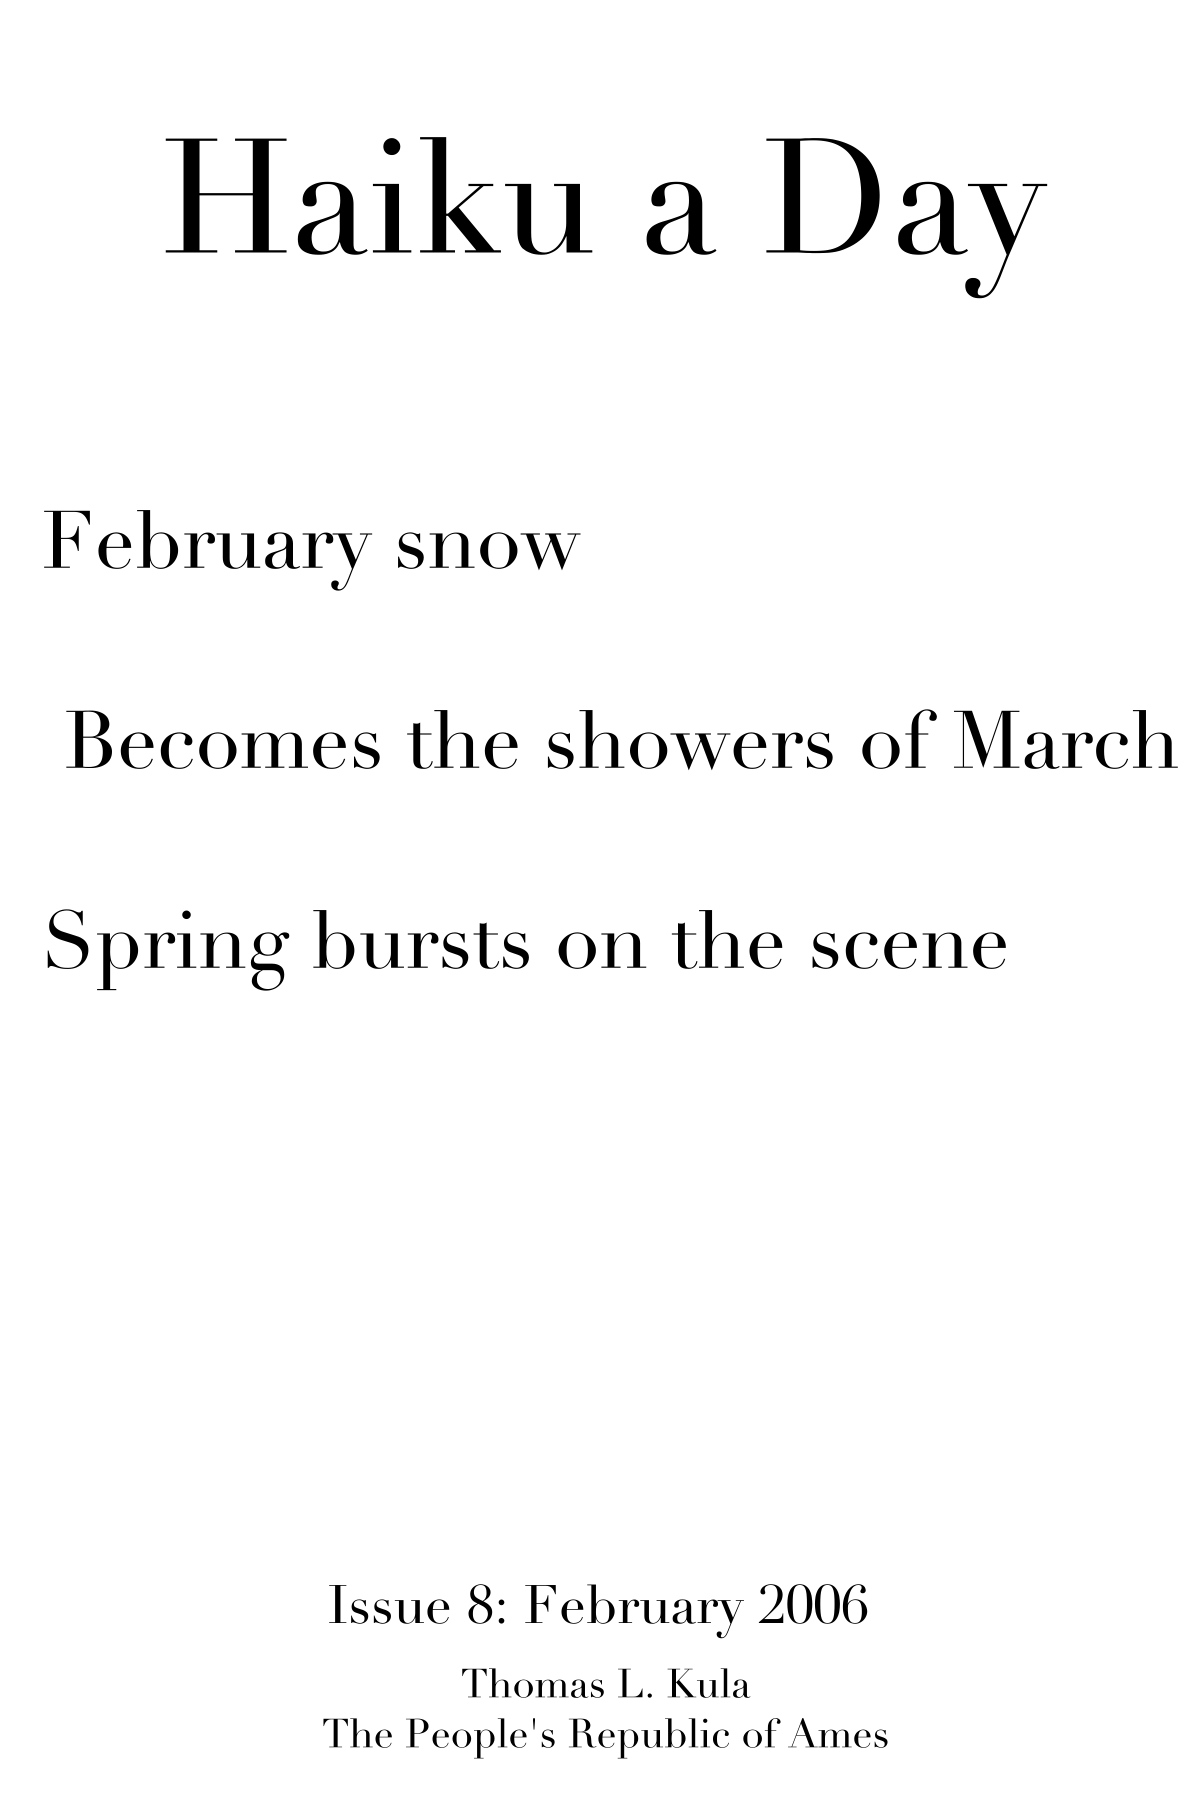
\includegraphics[width=101mm]{frontpage.png}

\newpage

The weather here in Ames has finally seemed to swing around firmly
to Spring. This winter wasn't as harsh as others have been, but
we had some cold days, some warm days, back to cold. But in the
past couple of weeks we've gotten rain and little bits of hail,
and I'm starting to really look forward to spring.

Last weekend was KaleidoQuiz 2006, the 26 hour trivia marathon that
the radio station at ISU puts on. This year, I worked the radio
station side, which was amazingly fun. For those of you curious,
it only takes five people to pull an empty CyRide bus.

--- Thomas

P.O. Box 1124 \\
Ames, IA 50014-1124 \\
http://kula.tproa.net/had/

Downloadable version available at website, or if you really
want me to send you one, send me your address, maybe a
stamp too. I enjoy getting mail as much as I enjoy sending
mail.\\

\setlength{\parskip}{1mm}

\newpage

1 February 2006    

Babysit Regents \\
Their network is fine and the \\
Free food aint bad too.

2 February 2006

sadly work beckons \\
it's not as fun as a nap \\
but it pays the bills

3 February 2006

A boring Friday \\
My house is a mess and I \\
Feel like doing naught

4 February 2006

Cheese and tortillas \\
Throw in some taco seitan \\
Yum, quesadillas

5 February 2006

Hour of piping \\
Teaching begining students \\
Instructing is fun.

6 February 2006

Sending my taxes \\
Requires a stupid stamp \\
That's a bit unfair


\newpage

7 February 2006

The sky becomes grey \\
The air becomes cold and still \\
Snow is upon us

8 February 2006

I buy surplus junk \\
More stuff to clutter my house \\
Need more computers

9 February 2006

My house is a mess \\
Junk clutters my living room \\
I should throw it out.

10 February 2006

City Hall to Mall \\
Walking that takes less time than \\
One would expect it

11 February 2006

That walk made me sore \\
But gave an epiphany \\
In a better mood.

12 February 2006

I miss hearing the \\
Sunday Morning Polka Show \\
Grandma's radio


\newpage

13 February 2006

My house is dirty \\
But a flurry of action \\
Makes it a bit clean

14 February 2006

Goulash of the Gods \\
Tastier the second day \\
And my house smells nice

15 February 2006

Brief hail of pellets \\
A signal of impending snow \\
Grey skies await us

16 February 2006

Shovel right away \\
Driveway is clean after work \\
Where is the real me?

17 February 2006

Morning sky grows bright \\
Earlier than I expect \\
Spring will soon be here

18 February 2006

The harsh wind at noon \\
Makes me think we should rename: \\
Ames, Siberia


\newpage

19 February 2006

My potato soup \\
Tasty, but a little bland \\
More flavor next time.

20 February 2006

The week starts off bad \\
And in a bad mood I get. \\
Is it Friday yet?

21 February 2006

Idiots galore \\
Why do I know more than those \\
Paid more than I am?

22 February 2006

Library hangout \\
I need a little office \\
That would kick some ass

23 February 2006

Nude mathematics \\
A pornography niche that \\
Really needs filling

24 February 2006

You ignore your flag \\
I'm not the one who leaves it \\
Spattered, tattered, torn.


\newpage

25 February 2006

Pulling CyRide bus \\
It only takes five people \\
So we'll give them six

26 February 2006

The weather grows nice \\
Are we close to springtime now? \\
When will flowers grow?

27 February 2006

Rail grinder goes by \\
A Hades of sparks shoots out \\
A sinew of light.

28 February 2006

Payday, sweet payday \\
I am rich for one short day \\
Then bills take away

\newpage


\includegraphics[width=101mm]{backpage.png}

\end{document}




